	\documentclass[fleqn,10pt]{wlscirep}
\usepackage{tablefootnote}
\usepackage{threeparttable}
\usepackage{rotating}
\usepackage{booktabs}
\begin{document}
\title{Accurately Assessing The \textit{Global} Quality of NMR-derived RNA Structures Using Chemical Shifts}
\author[1,2*]{Aaron T. Frank}
\author[3]{Jingru Xie}
\affil[1]{University of Michigan, Department of Biophysics, Ann Arbor Michigan, 48109, USA}
\affil[2]{University of Michigan, Department of Chemistry, Ann Arbor Michigan, 48109, USA}
\affil[3]{University of Michigan, Department of Physics, Ann Arbor Michigan, 48109, USA}
\affil[*]{afrankz@umich.edu}
\keywords{Keyword1, Keyword2, Keyword3}
\begin{abstract}
NMR spectroscopy has emerged as a powerful tool for determining the complex architecture of non-coding RNAs, but assessing the quality of NMR-derived structures remains problematic in the field of RNA structural biology. We demonstrate that chemical shifts can serve as conformational ``fingerprints'' that can accurately assess the \textit{global} quality of NMR structures of RNA. This was accomplished by carefully comparing observed and computed chemical shifts for pairs of NMR structures of the same RNA, one of which is known to be more accurate representation of the solution state structure of the RNA than the other. We discovered that in each of the five cases that were examined, we were able to correctly identify the more ``accurate'' NMR structure when using the chemical shift error as a quality-factor. The promising results described in this report should pave the way for the development of tools that utilize chemical shifts to assess the global quality of NMR structures of RNA. As an initial step in this direction, we developed a graphical analysis and quality assessment tool, PyShifts, which we make freely available at https://github.com/atfrank/PyShifts. 
\end{abstract}
\flushbottom
\maketitle
% * <john.hammersley@gmail.com> 2015-02-09T12:07:31.197Z:
%
% Click the title above to edit the author information and abstract
%
% ^ <afrankz@umich.edu> 2016-08-13T04:05:37.998Z.
\thispagestyle{empty}
\section*{Introduction}
The ever-increasing regulatory roles attributed to non-coding ribonucleic acids (RNAs) has resulted in keen interest in characterizing the atomistic structure of these functional biomolecules \cite{storz2002expanding}. Determining their structure using X-ray crystallography is complicated by that fact that extensive interactions can formed between lattices. For small RNAs, in particular, these lattice interactions are known to strongly modify their structure, rendering the crystal structure  unrealistic ``picture''  solution state of an RNA. NMR spectroscopy has emerged as a powerful tool for determining the solution structure of an RNA, either by itself or when interacting with other biomolecules and ligands. However, NMR ensembles may not be reliable representation of the solution state of an RNA due, in part, to sparsity of long-range structural restraints and sensitivity to modeling parameters and optimization protocols  employed when calculating and refining structures. As such, there is a need for methods that enable the quality of an NMR-derived structure of RNA to be accurately assessed. Unfortunately, accurately assessing the quality of NMR-derived RNA structures remains a challenge \cite{montelione2013recommendations}. As an atomic-level conformational ``fingerprint,'' NMR-derived chemical shifts can theoretically be used to uniquely identify RNA conformational state. Chemical shifts should therefore be useful in assessing the quality of NMR structures of RNA. In the context of quality assessment, one would expect that low-quality models that contain significant structural errors should be less compatible with the available chemical shift data than more accurate structural models. This idea is bolstered by recent work demonstrating that non-exchangeable $^{1}$H chemical shift data can be used to disambiguate energetically similar yet distinct RNA conformations \cite{sripakdeevong2014structure}. This strongly suggests that chemical shift data should also be useful for assessing the quality of RNA structures, similar to their utility in examining protein structure quality \cite{vila2009assessing, sahakyan2011using, sahakyan2012protein, martin2013physics, zhu2014correction}. Furthermore, because chemical shifts are not \textit{directly} used in determining the NMR structures of RNA, they represent an independent and orthogonal source of information, and as such, any validation method that \textit{directly} utilizes chemical shifts to assess RNA structure quality would constitute a ``strong'' validation method \cite{vila2009assessing}. 

To be useful in quality assessment, theoretical and computational methods must exist that enable chemical shifts to be rapidly and accurately computed from 3-dimensional (3D) RNA coordinates so that they can be compared to observed chemical shifts. In addition to first-principle methods, several empirical structure-based approaches have been developed that enable $^{1}$H, $^{13}$C, and $^{15}$N chemical shifts to be predicted from 3D coordinates of RNAs\cite{dejaegere1999empirical,cromsigt2001prediction, frank2013prediction,frank2014simple, frank2016can}. Therefore, the predictive tools needed to efficiently compute chemical shifts from RNA atomic coordinates are in place; what is currently lacking is a systematic analysis of the extent to which a comparison between observed and computed chemical shifts can, within the prediction errors of these methods, be used to accurately assess the quality of related NMR structures of the same RNA. More specifically, given a set of experimental assigned chemical shift data (e.g. $^{1}$H and $^{1}$C chemical shifts) of an RNA and associated chemical shifts computed from a set of NMR-derived structures, can the error between observed and computed chemical shifts can be used to assess the global quality of the individual structures?

One strategy towards answering this question would be to demonstrate that the error between observed and computed chemical shift can be used to discriminate between sets low and higher accuracy experimental structures of individual RNAs.  Such an analysis, however, is complicated by the fact that any error between observed and computed chemical shifts can have two sources:  errors in the experimental structure and errors in the computed chemical shift. Though it is impossible to completely resolve these two sources of error, one could still establish the chemical shift errors as a useful quality metric by examining RNAs for which pairs of lower and higher ``confidence'' structures of the same RNA are available, and for which experimental chemical shift data is available. For a number of RNAs in the PDB for which chemical shift data is available, both ``obsolete'' and ``refined'' NMR structure available (see Table \ref{tab:testcases}). In most of these cases, the original (and now obsolete)  structure was refined using additional NOEs and newly acquired RDC data, and it is reasonable to assume that these structure are better representations of the solution state of these RNAs. As such, these pair of ``outdated'' and ``updated'' structures for these RNAs provide an excellent opportunity to examine the utility of chemical shifts data can be used to assess the relative global quality of NMR-derived structures.

%\begin{table}[h]
%\centering
%\begin{threeparttable}
%\begin{tabular}{c c c c c c c c c}
%\hline
%\\
%Test & RNA name & \tnote{a} \ PDB identifiers & \tnote{b} \ RMSD (\AA) & \tnote{c} \ RMSF (\AA)   & \tnote{d} \ No. Chemical Shifts & Original Restraints & Refinement \\
%\\
%\hline
%\\
%1 & Domain 5 yeast ai5($\gamma$) group II intron & 1R2P:2LPS & 4.76   & 0.70 & 220/89 & 678/261/72/24 & restrained MD simulations using original NMR restraints () \\
%2 & Helix II template boundary element & 2FRL:2M22 & 4.48  & 0.89 & 175/151  \\
%3 & Stem IV terminal loop & 2H2X:2M21 & 5.00 & 0.93  & 164/141  \\
%4 & PreQ$_{1}$ riboswitch aptamer & 2KFC:2L1V & 1.90  & 0.61 & 270/229   \\
%5 & Tetrahymena telomerase RNA pseudoknot  & 2N6Q:5KMZ & 1.81  & 0.23 & 150/80 \\
%\\
%\hline
%\end{tabular}
%\begin{tablenotes}
%\item[a] PDB identifiers for the pair of NMR structures in each test case. The former and latter identifiers correspond to the ``outdated'' and ``updated'' NMR structures, respectively.
%\item[b] structural root mean squared distance (RMSD) calculated between the average coordinate of the pair of NMR structures
%\item[c] the average residue-wise root mean squared fluctuation within updated NMR ensemble
%\item[d] number of $^{1}$H/$^{13}$C non-exchangeable assigned chemical shifts 
%
%\end{tablenotes}
%\end{threeparttable}
%\caption{\label{tab:testcases} Test cases used to examine the ability of chemical shifts to assess the \textit{global} quality of NMR-derived RNA structures.}
%\end{table}
%

\begin{table}[h]
\centering
\begin{threeparttable}
\begin{tabular}{c c c c c c c c }
\hline
\\
RNA name & \tnote{a} \ PDB identifiers & \tnote{b} \ RMSD \ / \tnote{c} \ RMSF (\AA)  &  \tnote{d} \ Original Restraints & \tnote{d} \ New Restraints \\
\\
\hline
\\
(1) Domain 5 yeast ai5($\gamma$) group II intron & 1R2P:2LPS & 4.76  \ / \ 0.70 & 596 \ / \ 263 \ / \ 24 & same \\
(2) Helix II template boundary element & 2FRL:2M22 & 4.48  \ / \ 0.89& 517 \ / \ 162 \ / \ 25 & 518 \ / \ 163 \ / \ 63  \\
(3) Stem IV terminal loop & 2H2X:2M21 & 5.00 \ / \ 0.93& 452 \ / \ 168 \ / \ 0 & 496 \ / \ 151 \ / \ 53    \\
(4) PreQ$_{1}$ riboswitch aptamer & 2KFC:2L1V & 1.90 \ / \ 0.61& 815 \ / \ 154 \ / \ 0 & 814 \ / \ 154 \ / \ 76   \\
(5) Tetrahymena telomerase RNA pseudoknot  & 2N6Q:5KMZ & 1.81 \ / \ 0.23 & 499 \ / \ 174 \ / \ 77  & same  \\
\\
\hline
\end{tabular}
\begin{tablenotes}
\item[a] PDB identifiers for the pair of NMR structures in each test case. The former and latter identifiers correspond to the ``outdated'' and ``updated'' NMR structures, respectively.
\item[b] structural root mean squared distance (RMSD) calculated between the average coordinate of the pair of NMR structures
\item[c] the average residue-wise root mean squared fluctuation within updated NMR ensemble
\item[d] No. of NOE / Dihedral / RDCs restraints used during structure calculations

\end{tablenotes}
\end{threeparttable}
\caption{\label{tab:testcases} Test cases used to examine the ability of chemical shifts to assess the \textit{global} quality of NMR-derived RNA structures.}
\end{table}

Below, we describe our efforts centered on testing the hypothesis that the \textit{global} quality of NMR-derived structures could be accurately assessed by comparing observed chemical shifts with chemical shifts computed from NMR structures. To do this, we carried out five independent tests, in which a set of actual, experimentally observed chemical shifts  was used to assess the quality of a pair of solved structural models of a given RNA (Table \ref{tab:testcases}). For each RNA in our five test cases, one of the NMR structures corresponded an less refined and now ``outdated'' NMR structure, and the other,  corresponded to more refined, updated NMR structure. We discover that, in general, the structures from the updated NMR ensemble exhibited lower errors between observed and computed chemical shifts than the structures taken from the outdated (and less accurate) NMR ensemble.

\section*{Methods}
\subsection*{Experimental NMR structures and chemical shift data}
We compiled a dataset consisting of five RNAs for which NMR chemical shifts were available in the BMRB \cite{ulrich2008biomagresbank} and for which two set of NMR structures existed in the PDB \cite{bernstein1978protein}, one corresponding to the originally deposited NMR and the other to a more accurate, updated, and refined NMR structure. Specifically, our dataset contained the outdated (``obsolete'') and updated structures of the preQ1 riboswitch (PDB:2KFC, PDB:2L1V; BMRB:17106) \cite{zhang2011comparison,kang2009structural}, the yeast ai5($\gamma$) group II intron RNA (PDB:1R2P, PDB:2LPS; BMRB:5962) \cite{henriksen2012molecular,sigel2004solution}, the Tetrahymena telomerase stem IV terminal loop RNA (PDB:2H2X, PDB:2M21; BMRB:18891) \cite{richards2006structural}, the helix II template boundary element from Tetrahymena telomerase RNA (PDB:2FRL, PDB:2M22; BMRB:18892) \cite{richards2006structure}, and the Tetrahymena telomerase RNA pseudoknot (PDB: 2N6Q, PDB: 5KMZ; BMRB: 25777)\cite{jiang2015structure}.

\subsection*{Computing chemical shifts from structural models}
For each of the five RNAs in our testing set, $^{1}$H and $^{13}$C non-exchangeable chemical shifts were computed using LARMOR$^{\rm D}$ \cite{frank2014simple} and RAMSEY \cite{frank2013prediction}, two empirical structure-based predictors.  LARMOR$^{\rm D}$ and RAMSEY computed chemical shifts were also used to calculate a ``consensus'' prediction for each nuclei. Consensus computed chemical shifts were then determined by calculating the mean of the LARMOR$^{\rm D}$ and RAMSEY computed chemical shifts. Accordingly, three sets of analyzes were carried out using RAMSEY, LARMOR$^{\rm D}$, and consensus computed chemical shifts. 

\subsection*{Assessing the quality of NMR structures} 
To assess the quality of NMR structures, we computed the weighted (or reduced) mean-absolute-error between the observed and computed chemical shifts, using the expression:
\begin{equation}\label{eq:Q} 
$w$MAE = \frac{1}{N} \sum_{i=1}^{N} \mathit{w_{i}} | \delta_{\rm obs,i} - \delta_{\rm comp,i} |,
\end{equation}
where $\delta_{\rm obs,i}$ and $\delta_{\rm pred,i}$ are the observed and predicted chemical shifts, respectively; $N$ is the number of chemical shifts; and $w_{i}$ is a weight factor that is equal to $1/\sigma_{i}$, where $\sigma_{i}$ is the expected accuracy of predictions for the nucleus type associated with $i^{th}$ chemical shift data point. For both LARMOR$^{\rm D}$ and RAMSEY, $\sigma_{i}$ values were determined from the analysis of their respective prediction errors on datasets that were independent of the data used to train the predictive models on which they are based. 

We utilized three sets of analyzes to assess whether errors between observed and computed chemical shifts can be used to assess the global quality of the outdated and updated of NMR structures in each of the five test cases examined in this study: (1) For each test case, the average structure of the outdated and the average structure of the updated NMR ensembles were determined, and the resulting structure energy minimized using the CHARMM36 RNA force field. Energy minimization was carried out the CHARMM molecular dynamics simulation package. LARMOR$^{\rm D}$, RAMSEY, and consensus chemical shifts were then computed from these energy-minimized structures, and the error between observed and computed chemical shifts were then determined; (2) LARMOR$^{\rm D}$, RAMSEY, and Consensus chemical shifts were computed from all of the structures in the outdated and all of the structures in the updated NMR ensembles. Next, computed chemical shifts were conformationally averaged. More specifically, for the set of chemical shifts computed from the outdated ensemble and the updated ensemble, the chemical shift for a given nuclei was calculated as the average of the chemical shifts obtained from each structure in the corresponding ensemble. For a given ensemble, structures were equally weighted. Finally, for each test case, the error between observed chemical shifts and the conformationally averaged computed chemical shifts was determined for the outdated and updated NMR ensemble, respectively. (3) LARMOR$^{\rm D}$, RAMSEY, and consensus chemical shifts were computed from all of the structures in the outdated and all of the structures in the updated NMR ensembles.  The error between observed chemical shifts and chemical shifts computed from each structure in the outdated and updated NMR ensemble, respectively, were then calculated.

\subsection*{Assessing the ability of computed chemical shifts to resolve individual NMR structures in the composite ensemble} In addition to determining whether the which NMR ensemble (outdated or updated) exhibited the lowest error between observed and computed chemical shifts, in the last approach described above, we were interest in examining whether errors between observed and computed chemical shifts could used to discriminate between the structures in the outdated and updated chemical shifts. More specifically, were interested in answering the examining whether  the structures in updated ensemble tended to have lower errors than the structures in the outdated NMR ensemble.  As in previous work, we used the NSLR metric\cite{Venkatraman:2010gea} to assess the ability of the chemical shift errors to resolve individual NMR structures in the outdated and updated NMR ensembles. Briefly, the NSLR is an early recognition metric in a binary classification problem \cite{Venkatraman:2010gea} that ranges from 0 to 1, where 1 corresponds to the highest resolving power. The NSLR is expressed as 
\begin{equation}\label{eq:NSLR} 
{\rm{NSLR} }= \frac{\rm{SLR}}{\rm{SLR}_{\rm max}}
\end{equation}
where the SLR is calculated as
\begin{equation}\label{eq:SLR} 
{\rm{SLR}} = - \sum_{i=1}^{n} \log{\frac{r_{i}}{N}}
\end{equation}
where (within the current context) $r_{i}$ is the rank of the $i^{th}$ structure in the ``updated'' ensemble when models are sorted (in ascending order) based on the chemical shift errors, $n$ is the total number of structures in the ``updated'' ensemble, $N$ is the total number of structures in the outdated and updated NMR ensembles, and SLR$_{\rm max}$ is the theoretical maximum value of the SLR. SLR$_{\rm max}$ is achieved when all $n$ native poses are ranked within the first $n$ position. SLR$_{\rm max}$ is calculated as 
\begin{equation}\label{eq:SLRmax} 
{\rm{SLR}_{\rm max}} = - \sum_{i=1}^{n} \log{\frac{i}{N}}
\end{equation}

\subsection*{Determining importance of individual non-exchangeable $^{1}$H and $^{13}$C nuclei in discriminating outdated NMR structures from updated NMR structures} To gain some insight into which non-exchangeable $^{1}$H and $^{13}$C RNA nuclei are better at  discriminating between structures from an outdated NMR ensembles and structures from an updated NMR ensembles, we used a machine learning based feature selection approach. To do this, we cast the problem of discriminating between outdated and updated structures as a classification problem in which the features used to ``classify'' a structure as outdated or updated are the errors between observed and computed chemical shifts for individual non-exchangeable $^{1}$H and $^{13}$C RNA nuclei. Using the chemical shift errors as ``features'', a classification model could be trained and then the importance of the individual features to the classification model can be determined. In so doing, the importance of each nuclei in discriminating between outdated and updated structures could be determined. To build such a classification model, we generated a training database in which each sample (or datapoint) corresponds to one of the structures from the outdated and updated NMR structure in our five testing set (see above). For each such sample (structure), we determined the mean error between observed and computed chemical shift for each type of 19 non-exchangeable $^{1}$H and $^{13}$C RNA nuclei, namely,  H1', H2', H3', H4', H5', H5'', H2, H5, H6, H8, C1', C2', C3', C4', C5', C5'', C2, C5, C6,  and C8 nuclei, respectively. As such, each sample had 19 features, and was classified as 0 and 1 if the structure from which the error features were calculated belonged to the outdated or updated NMR ensemble, respectively.  Using the resulting training database, the random forest technique was then used to build a classification model, and the importance of individual features to the classification model determined. Three separate classification models were generated using LARMOR$^{\rm D}$, RAMSEY, and consensus chemical shift errors as features.

\subsection*{Assessing the sensitivity of computed chemical shifts to structural changes in RNA} In order to investigate the sensitivity of computed chemical shifts to structural changes in RNA, we again utilized a feature selection approach to determine which set of structural features were most important for accurately predicting chemical shifts. To do this, a set of random forest predictive models were generated that were trained to predict LARMOR$^{\rm D}$, RAMSEY, and Consensus chemical shifts, based on certain structural features believed to be important for modeling shielding effects in RNAs.  In particular, predictive models were built that used a descriptors that contained information about close contacts, ring current, magnetic anisotropy and bond polarization effects, base--base  hydrogen bond, base-backbone  hydrogen bond, backbone--backbone hydrogen bond and base--base stacking, and the backbone, ribose and the glycosidic dihedrals. To focus our analysis on structural changes relevant to the RNAs the five RNAs in our test set, we first used steered molecular dynamics (SMD) to generate transition pathways between the average outdated and the average updated NMR structures of each of the five RNAs we studied. From the resulting structures, chemical shifts were computed using LARMOR$^{\rm D}$ and RAMSEY. Consensus chemical shifts were also determined as the mean of LARMOR$^{\rm D}$ and RAMSEY predictions. The structural descriptor (see above) were then extracted from the resulting structures along the trajectories, and then mapped to the chemical shifts computed from the structures to compile a final training database. As in previous work, the structural descriptors were extracted structures using an in-house Python script, written using MDAnalysis\cite{michaud2011mdanalysis}. Random forest predictive models were then generated separately for every non-exchangeable proton (H1', H2', H3', H4', H5', H5'', H2, H5, H6, and H8) and carbon (C1', C2', C3', C4', C5', C2, C5, C6, and C8) nucleus that attempted to reproduce LARMOR$^{\rm D}$, RAMSEY, and Consensus chemical shifts computed from the structures along the transition pathways between the outdated and updated NMR structures in our test set. From each predictive model, the importance of each descriptor was then determined. Briefly, the importance of a given descriptor is determined by quantity the increase in the prediction that occurs when that data corresponding to that descriptor (and only that descriptor) is randomly permuted throughout the training database. Using this approach, the importance of each descriptor was determined.


%To overcome this limitation, we once again utilized a feature selection approach to determine--in a manner similar to the approach we used above to determine the importance individual nuclei for discriminating outdated NMR structures from updated structures--the importance of individual structural features, in particular, those are most relevant to describing structural changes  in the RNAs and those that are typically used to modeling electronic shielding effects. In particular, we used a machine learning approach to build predictive models which from we are able to learn the \textit{implicit} importance of specific structural features, even though, as is the case for LARMOR${\rm D}$, these features are not explicitly used in predicting chemical shifts. Briefly, predictive models trained, using the random forest approach, to recapitulate either Consensus, LARMOR${\rm D}$, or RAMSEY \textit{computed} chemical shifts and then we determined the importance of individual structural features. For these predictive models, structural features corresponded to residue level features like hydrogen, base-stacking, torsion dihedral, ribose dihedrals and glycosidic dihedral, and atom level feature like ring currents, magnetic anisotropy, and bond polarization effect. To focus our analysis, the training set used to build these models corresponded to chemical shifts and structure features computed from transition path trajectories that were generated using the average structure of outdated and the updated NMR ensembles for each RNA in our testing set as endpoints. In so doing, we were able to probe the sensitivity of computed chemical shifts to individual structural features.

%All the analyses described in this report were carried out using R, and a git repo that contains all the analysis scripts and primary data used in this report accompanies this manuscript (https://github.com/atfrank/global$\_$quality$\_$assessment).

\section*{Results and Discussion}
\begin{figure}[h]
\begin{center}
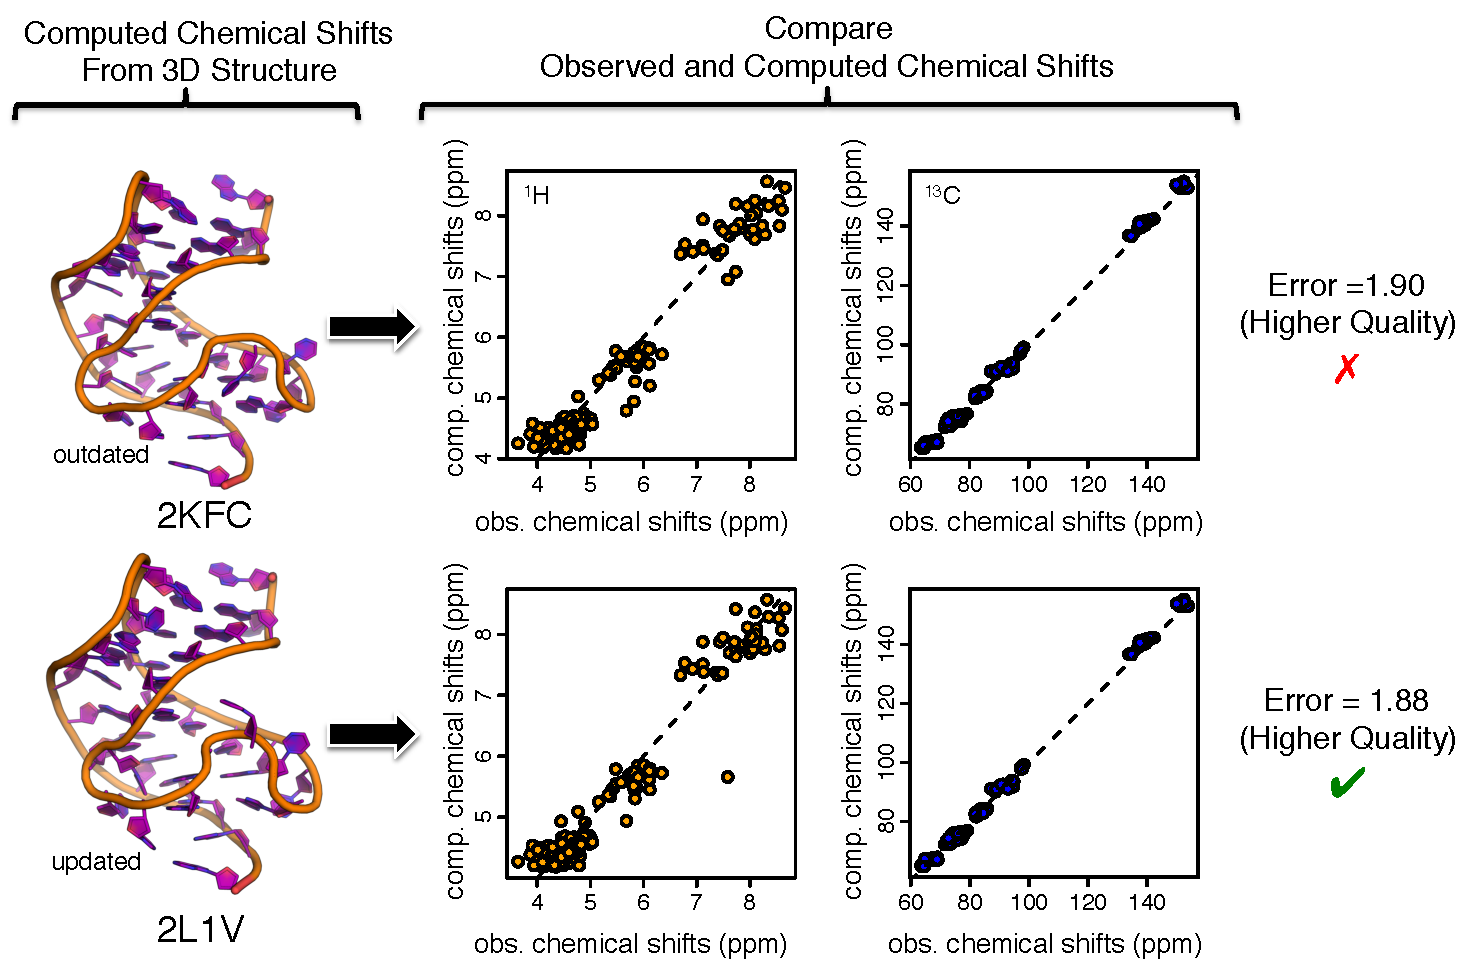
\includegraphics[width=0.8\textwidth]{figure_illustrate}
\end{center}
\caption{Illustrating the use of chemical shifts to assess the \textit{global} quality of NMR-derived RNA structures. First, chemical shifts were computed from 3D coordinates of the RNAs. Next, the error between observed and computed chemical shifts was determined. The model that exhibited the lowest chemical shift error was identified as the higher quality structure. This is illustrated in this figure by comparing observed chemical shifts with those computed from the average coordinate of the outdated NMR structure (PDB: 2KFC; top) and updated NMR structure (PDB 2L1V; bottom), respectively, for the preQ$_{1}$ riboswitch aptamer.}
\label{fig:illustrate}
\end{figure}

If our working hypothesis is correct, namely, that chemical shift errors can be used to accurately assess the \textit{global} quality of NMR structures, we would expect that in each of the five test cases we examined (see Table \ref{tab:testcases}) the model(s) that exhibited the lowest error between the observed and computed chemical shifts would be model(s) that belong to the ``updated'' NMR structure. This expectation is based on the fact for each of the five RNAs, the updated structure either better satisfied the available NMR restraints (RNA 1 and 5; see Table \ref{tab:testcases}) or was calculated using additional NMR restraints that included residual dipolar couplings (RDCs), which are source of long range structural information (RNA 2, 3, and 4; see Table \ref{tab:testcases}) and are known to improve the fidelity of resulting NMR structures. As such, it is assumed that overall, the updated structures are a more accurate representation of the solution state structure of each of these RNAs. Here, of course, we also implicitly assume (1) that the information contained in observed chemical shifts can be used as conformational signatures of RNAs and (2) that chemical shifts can be computed from structures of RNAs with sufficient accuracy that enables the chemical shift error to be used as a robust ``quality factor''.

To directly test our hypothesis, we carried out three sets of analyzes. In the first instance, chemical shift errors were calculated between the observed chemical shifts and chemical shifts computed from the average structure of the outdated and updated NMR structures. Secondly, chemical shifts errors were calculated between the observed chemical shifts and conformationally-averaged chemical shifts that were obtained by determining, for each nuclei, the average computed chemical chemical shift over the structures in the outdated and updated ensembles, respectively. Finally, we computed chemical shift errors for each structure in the outdated and updated NMR bundles, and then for each, determined the chemical shift error. In each case, to quantify the overall ability of chemical shift errors to assess the \textit{global} quality of NMR structures, we determined the fraction of cases for which the lowest error model belonged to ``updated'' NMR structure. 
\begin{table}[h]
\centering
\begin{threeparttable}
\begin{tabular}{c c c c c}
\hline
\\
Prediction Method  & \tnote{a} \ Average Structures & \tnote{b} \ Conformationally-Averaged Chemical Shifts &  \tnote{c} \ Individual Models \\
\\
\hline
LARMOR$^{\rm D}$ & 0.6/0.8/0.8 & 0.8/0.8/0.8 & 0.8/0.6/0.6 \\
RAMSEY & 0.8/1.0/1.0 & 1.0/1.0/1.0 & 1.0/1.0/1.0 \\
Consensus & 0.8/1.0/1.0 & 0.8/1.0/1.0 & 1.0/0.8/1.0 \\
\hline
\end{tabular}
\begin{tablenotes}
\item[a] Errors were calculated between observed chemical shifts and chemical shifts computed from the average structure of the outdated and updated NMR ensembles respectively. 
\item[b] Errors were calculated between observed chemical shifts and conformationally-averaged chemical shifts of the outdated and the updated NMR ensembles respectively. 
\item[c] Errors were calculated between observed chemical shifts and chemical shifts computed from each structural model in the outdated and updated NMR ensembles, respectively.
\end{tablenotes}
\end{threeparttable}
\caption{\label{tab:tpr} Quanitying whether lowest error models belong to the updated NMR structures. Listed are the fraction of cases (over the five cases we examined) for which the lowest error model belonged to the updated (and more refined) NMR ensemble.}
\end{table}

\subsection*{Updated NMR structures exhibit better agreement between observed and computed chemical shifts than the outdated NMR structures.} 

We began our analysis by examining errors between observed chemical shifts and chemical shifts computed from the average structure of the outdated and updated NMR ensembles of each our five test cases. We found that in general, the average structure of the updated NMR ensemble exhibited better agreement between observed and computed chemical shifts than the average structure of the outdated NMR ensemble (Table \ref{tab:tpr}). For example, when prediction chemical shifts using LARMOR$^{\rm D}$, the fraction of cases in which the updated structure exhibited the best agreement were 0.6 (3/5), 0.8 (4/5), and 0.8 (4/5), when using only $^{1}$H, $^{13}$C, and both $^{1}$H and $^{13}$C, respectively (Table \ref{tab:tpr}). If instead chemical shifts were computed using RAMSEY, these values were slightly higher:  0.8 (4/5), 1.0 (5/5), and 1.0 (5/5), when using only $^{1}$H, $^{13}$C, and both $^{1}$H and $^{13}$C, respectively; similar results  were obtained using the LARMOR$^{\rm D}$-RAMSEY consensus chemical shifts (Table \ref{tab:tpr}).

%Were the errors in chemical shifts generally in regions that exhibited significant structural discrepancies?

Next, we repeated the above analysis, however, instead of using chemical shifts computed from the average structure of the outdated and updated NMR ensembles, we used the conformationally-averaged chemical shifts for each to calculate the chemical shift errors. When calculating conformationally-averaged chemical shifts for each ensemble, each model in the ensemble was equally weighted. Using these sets of conformationally-averaged chemical shifts, we obtained results that were similar to those obtained using chemical shift computed from the average structures of the outdated and updated NMR ensembles. In this case, for LARMOR$^{\rm D}$, the fraction of cases in which the updated structure exhibited the best agreement were 0.8 (4/5), 0.8 (4/5), and 0.8 (4/5), when using only $^{1}$H, $^{13}$C, and both $^{1}$H and $^{13}$C, respectively (Table \ref{tab:tpr}). By comparison these values were  0.8 (4/5), 1.0 (5/5), and 1.0 (5/5)  and 0.8 (4/5), 1.0 (5/5), and 1.0 (5/5) when using RAMSEY and LARMOR$^{\rm D}$-RAMSEY consensus chemical shifts, respectively (Table \ref{tab:tpr}).

Rather than restricting our comparison to pairs of observed and computed chemical shifts as done above, we next calculated the errors between observed chemical shifts and chemical shifts computed from each model in the outdated and updated NMR ensembles, respectively. We then, for each test case, determined whether or not the lowest model belonged to the outdated ensemble or the updated ensemble. Overall, similar result were obtained. In this case, for LARMOR$^{\rm D}$, the fraction of cases in which the updated structure exhibited the best agreement were 0.8 (3/5), 0.6 (3/5), and 0.6 (3/5), when using only $^{1}$H, $^{13}$C, and both $^{1}$H and $^{13}$C, respectively (Table \ref{tab:tpr}), compared to  1.0 (5/5), 1.0 (5/5), and 1.0 (5/5)  and 1.0 (5/5), 1.0 (5/5), and 1.0 (5/5) when using RAMSEY and LARMOR$^{\rm D}$-RAMSEY consensus chemical shifts, respectively (Table \ref{tab:tpr}).

\begin{figure}[h]
\begin{center}
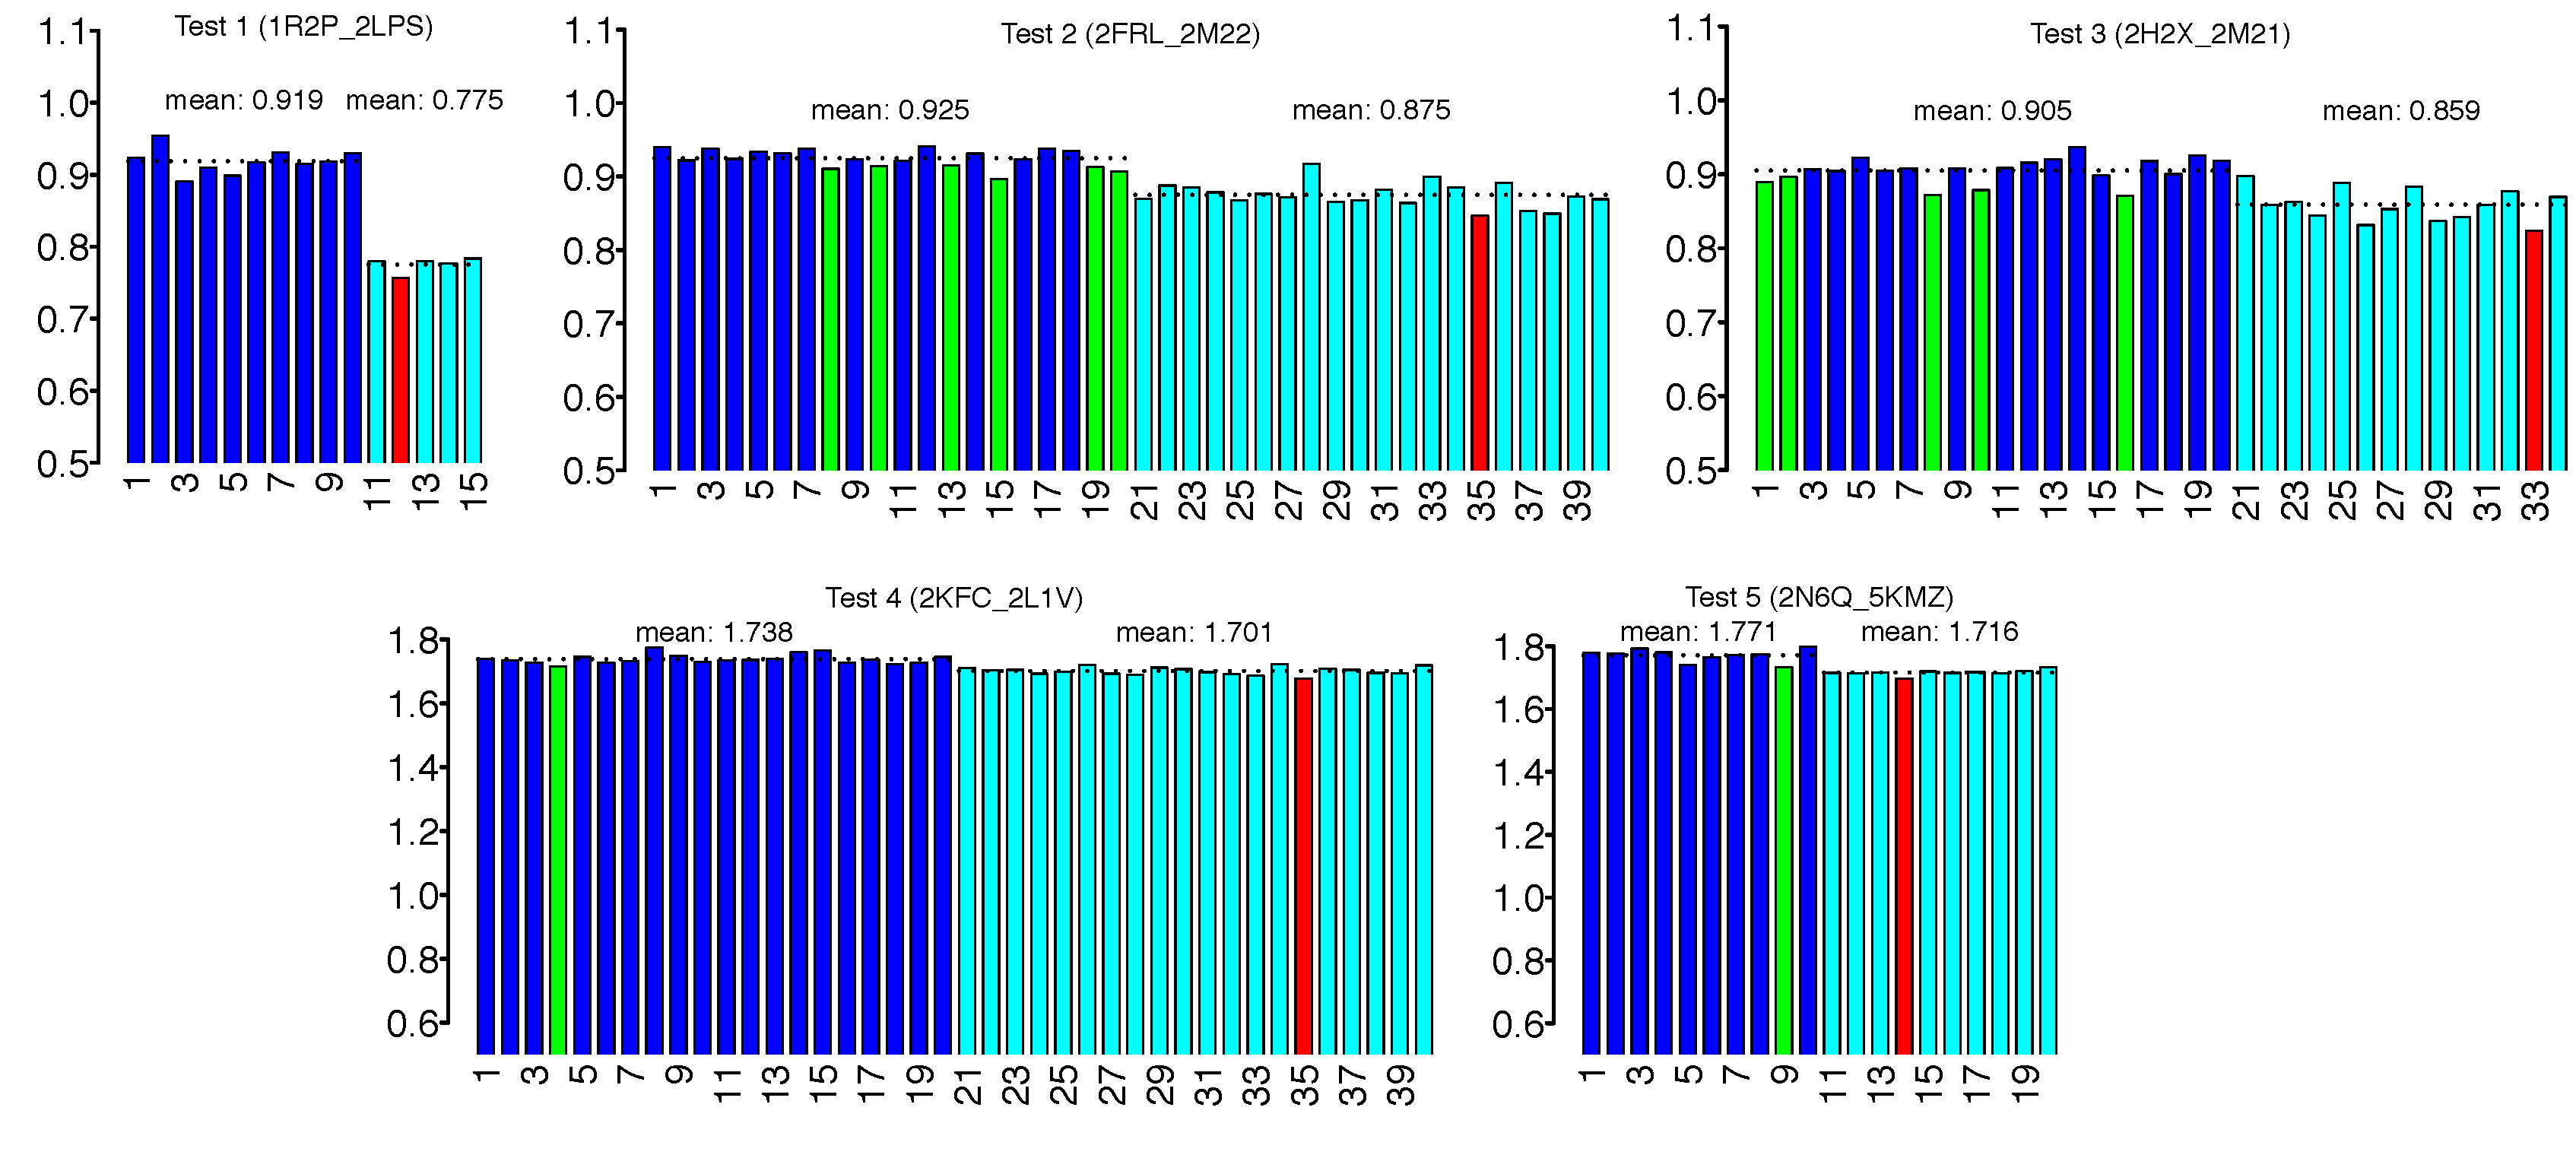
\includegraphics[width=0.8\textwidth]{figure_error_bars}
\end{center}
\caption{Comparing the chemical shift errors of structures in the outdated and updated NMR ensembles. For each test case, the barplot shows the chemical shift error for every model in the outdated (blue) and updated (cyan) NMR ensembles. For each test case, the structure with the lowest error is shown in red and the outdated models that exhibit errors the are lower than at least one of the updated models are shown green. Included in each barplot are the mean errors for models in the outdated and updated ensembles.}
\label{fig:errorbars}
\end{figure}

\subsection*{Chemical shift errors are able to separate structures belonging to the outdated NMR ensemble from those belonging to the updated NMR ensembles} The above results indicated that, in general, the updated structures appear to be more consistent with the available chemical shift data, as evidence by the fact that for each of the three set of analyzes, the lowest error structures tended to belong to the updated structure. However, though the ability to identify a ``updated'' structure as the lowest error model is a necessary condition for using chemical shift errors to robustly assess the quality of NMR structures, it is far from sufficient. For example, in a situation where there are $n$ outdated  structures and $m$ updated structure, even if the lowest error structure was one of the $m$ updated structures, the next $n$ lowest structures could all belong to the outdated NMR ensemble and the final $m-1$, to the updated ensemble. In this scenario, the above analysis would indicate that the lowest error model was from the updated ensemble, however, it says nothing about the overall ability of the chemical shift error to ``partition'' the outdated  and updated NMR ensembles.

To more closely compare the relative errors for individual models in the outdated and updated ensembles, we determined and then compared the mean chemical shift error for structures in the outdated to the mean chemical shift error of structures in the updated NMR structures. Figure \ref{fig:errorbars}, summarizes these results. For each of the five test cases, the mean chemical shift error of the updated NMR ensemble was lower than the outdated ensemble. However, for the preQ$_{1}$ riboswitch aptamer and Tetrahymena telomerase RNA pseudoknot RNAs (test 4 and 5, respectively) the difference were quite small; this, however, is due to the fact that structural difference between outdated and updated ensembles were also quite small; the RMSD between the average structure of the outdated and updated ensemble for the preQ$_{1}$ riboswitch aptamer and Tetrahymena telomerase RNA pseudoknot  RNAs were only 1.90 and 1.81 \AA, respectively (Table \ref{tab:testcases}). We did, however, notice that in 4 out of the 5 test cases, there were models in the outdated ensembles that exhibited chemical shifts errors that were larger than the chemical shift errors of some of the structures in the updated ensembles; for test 2 thru 5, we discovered 6, 5, 1, and 1 such model(s), respectively. Interestingly, the two RNAs contained the largest number of outdated models that exhibited structure chemical shifts errors less than some of the models in the updated ensemble, test 3 and 4, were also the RNAs exhibited the largest structural fluctuations within the updated ensemble, suggesting the updated NMR structures for these RNAs may be less restrained, and possibly slightly less accurate than the updated ensembles for the other RNAs. 

\begin{table}[h]
\centering
\begin{threeparttable}
\begin{tabular}{c c c c c}
\hline
\\
Test  & LARMOR$^{\rm D}$ & RAMSEY &  LARMOR$^{\rm D}$-RAMSEY & \tnote{a} \ Random\\
\\
\hline
1 & 1.00/1.00/1.00 & 1.00/1.00/1.00 & 1.00/1.00/1.00 & 0.49 \\
2 & 0.94/0.99/0.98 & 0.84/0.89/0.90 & 0.95/1.00/1.00 & 0.59 \\
3 & 0.79/0.64/0.75 & 0.84/0.82/0.87 & 0.98/0.81/0.96 & 0.53 \\
4 & 0.26/0.98/0.57 & 0.68/0.84/0.84 & 0.52/0.98/0.89 & 0.59 \\
5 & 1.00/0.20/1.00 & 1.00/1.00/1.00 & 1.00/0.81/1.00 & 0.59 \\
\hline
\\
mean & 0.80/0.76/0.86 & 0.87/0.91/0.92 & \textbf{0.89}/\textbf{0.92}/\textbf{0.97}  & 0.56\\
\\
\hline
\end{tabular}
\begin{tablenotes}
\item[a] Mean NSLR obtained after randomly ranking structures belonging to the outdated and updated NMR ensemble and then computing the NSLR.
\end{tablenotes}
\end{threeparttable}
\caption{\label{tab:nslr} Assessing the overall ability of chemical shift errors to discriminate between outdated and updated NMR structures. Listed are the NSLR values obtained when using $^{1}$H/$^{1}$C/$^{1}$H and $^{1}$C chemical shift errors to rank structures taken from the outdated and updated ensembles for each of the five RNAs examined here. Included are the result obtained using LARMOR$^{\rm D}$, RAMSEY, and LARMOR$^{\rm D}$-RAMSEY consensus chemical shifts. Here, values near one indicated that most of the structures in the updated ensemble exhibited lower chemical shift errors than the structures belonging to the outdated ensemble. }
\end{table}

These results notwithstanding, the fact that in each case (i) the lowest error structure belonged to the updated ensemble and (ii) the mean error of the over the structures in the updated ensemble were higher than the mean error over the structures in the outdated in indicated that chemical shifts error could, in general be used to separate the structures of the outdated and updated structures. To quantify this more directly, we computed the normalized sum of logarithmic ranks (NSLR, an early recognition metric) that quantifies the ability of a score (in our case, the chemical shift errors) to accurately partition two binary groups within a data set \cite{Venkatraman:2010gea} (in our case structures that belong to the outdated (0) and structures that belonged to the updated (1) NMR ensembles, respectively. The NSLR ranges between 0 and 1. In our test cases, NSLR would be equal to 0 if \textit{all} of $n$ models in the ``updated'' ensemble have the $n$ \textit{highest} chemical shift errors. Conversely, NSLR would be equal to 1 if \textit{all} $n$ models in the ``reference'' ensemble have the $n$ \textit{lowest} chemical shift errors (corresponding to the maximum resolving power). 

Using the NSLR as our resolving score, we discovered that the chemical shift errors were indeed able to resolve the pairs of NMR structures into separate groups (i.e., for most of the test cases, the NSLR values were close to 1; Table \ref{tab:nslr}). High resolving scores were particularly evident when both $^{1}$H and $^{13}$C chemical shifts were used to determine the errors (Table \ref{tab:nslr}). For comparison, we computed the best-case NSLR we would expect if \textit{random} errors were used to partition the models. We found that regardless of whether only $^{1}$H, $^{13}$C, or both $^{1}$H and $^{13}$C chemical shifts were used to determine the errors, the average resolving scores were significantly greater than this best-case random NSLR (Fig \ref{fig:nslr}c), demonstrating that the use of chemical shift errors to partition the NMR structure pairs in each test case was significantly better than what one would expect from random partitioning of the models in the ``reference'' and ``decoy'' NMR structures. Over the five test cases, chemical shift errors calculated using RAMSEY predicted chemical shifts were better able to separate structures belonging to the updated NMR ensemble from structures belonging to the outdated ensembles than errors calculated using LARMOR$^{\rm D}$ predicted chemical shifts. This result was consist regardless of whether $^{1}$H, $^{13}$C or both $^{1}$H and $^{13}$C were used to calculate the errors. Interestingly, the largest NSLR values were obtained when using LARMOR$^{\rm D}$-RAMSEY consensus chemical shifts (i.e, chemical shifts computed as the mean of LARMOR$^{\rm D}$ and RAMSEY predictions).

\subsection*{Removing prediction outliers enhances our ability to discriminate between outdated and updated NMR structures} As alluded to before, the use of chemical shift errors to assess the quality of NMR structures is complicated by the fact that in addition to structural differences between the outdated and updated NMR structures, the chemical shifts errors we calculated contain a contribution associated with the inherent errors of the predictors used to computed chemical shifts from structure. As such, to gain some  insights into the impact that prediction outliers have on the ability chemical shifts errors to discriminate between outdated and updated NMR structures, we carried out outliers analysis to identify potential outliers, eliminated these ``outliers'' and then calculated the mean NSLRs values over our five test cases. Here, we defined an ``outlier'' as a chemical shift data point for which the average scaled difference between observed and predicted chemical shifts, calculated over all the structures in the outdated and updated, is greater than some error threshold. The rationale here was that data points that exhibited large differences over all structures in both the outdated and updated structure were mostly likely outliers,  either due to errors in the reported chemical shifts or inherent flaws in chemical shift predictors. To explore this,  several sets of analyzes were carried out in which the error threshold, which was used to identify ``outliers'', was varied between 1 and 12. At each error threshold, we computed the NSLR for each test case and then calculated the average. In so doing, we were able to quantify the impact that prediction outliers had on our analysis.

\begin{table}[h]
\centering
\begin{threeparttable}
\begin{tabular}{c c c c c c c }
\hline
\\
\tnote{a} \ error threshold & LARMOR$^{\rm D}$ & RAMSEY  &  LARMOR$^{\rm D}$-RAMSEY\\
\\
\hline
\\
1      & 0.72 & 0.77 & 0.78 \\
2      & 0.81 & 0.83 & 0.93 \\
3      & 0.84 & 0.82 & 0.91 \\
4      & 0.86 & 0.84 & 0.92 \\
5      & 0.86 & 0.87 & 0.96 \\
6      & 0.85 & 0.91 & 0.95 \\
7      & 0.85 & 0.90 & 0.93 \\
8      & 0.84 & 0.90 & 0.93 \\
9      & 0.84 & 0.90 & 0.93 \\
10     & 0.85 & 0.90 & 0.93 \\
11     & 0.85 & 0.90 & 0.93 \\
12     & 0.81 & 0.90 & 0.93 \\                         
none   & 0.81 & 0.90 & 0.93 \\
\hline
\end{tabular}
\begin{tablenotes}
\item[a] Threshold used to determine outliers. For each test case, the average scaled difference between observed and computed chemical shifts was determined for data point over the combined outdated and updated ensembles, and data points with scaled errors greater than the threshold were removed prior to computing chemical shift errors and in turn the NSLRs.
\end{tablenotes}
\end{threeparttable}
\caption{\label{tab:outliers} Assessing the impact of prediction outliers. Listed are the mean NSLRs values obtained over the five cases using different error thresholds to identify and then remove outliers.}
\end{table}

Table \ref{tab:outliers} summarize the results of these analysis. In can be seen, we were able to identify a error threshold that resulted in an increase in the mean NSLR value for each of our chemical shift prediction methods. When using the LARMOR$^{\rm D}$, RAMSEY, LARMOR$^{\rm D}$-RAMSEY predicted chemical shifts, the most conservative error threshold that resulted in the largest mean NSLR were 5,  6, and 5 respectively (see Table \ref{tab:outliers}).  With these thresholds, the mean NSLR were 0.858,  0.908, and 0.961 respectively, compared with the values of  0.807, 0.901, and 0.927 that we obtained when we did not remove any outliers (see Table \ref{tab:outliers}). Interestingly, with an error threshold of 6, for example, only about 0.1\% of data points are identified as outliers (see Table \ref{tab:fraction_removed}). As such, these results indicate that by conservatively removing prediction outliers prior to calculating the chemical shift errors, we can enhance our ability to use chemical shift errors to discriminate the structural differences between the outdated and updated NMR structures in our test cases.

\begin{table}[h]
\centering
\begin{threeparttable}
\begin{tabular}{c c c c c c}
\hline
\\
nucleus & LARMOR$^{\rm D}$ & RAMSEY & LARMOR$^{\rm D}$-RAMSEY \\
\\
\hline
H1' & 0.723 & 0.216 & 0.222 \\
H2' & 0.250 & 0.241 & 0.162 \\
H3' & 0.210 & 0.147 & 0.183 \\
H4' & 0.541 & 0.355 & 0.524 \\
H5' & 0.482 & 0.617 & 0.244 \\
H5''& 0.451 & 0.322 & 0.275 \\
C1' & 0.210 & 0.215 & 0.099 \\
C2' & 0.373 & 0.213 & 0.241 \\
C3' & 1.000 & 0.355 & 0.567 \\
C4' & 0.140 & 0.182 & 0.200 \\
C5' & 0.260 & 0.458 & 0.265 \\
H2  & 0.897 & 0.293 & 0.476 \\
H5  & 0.181 & 0.764 & 0.506 \\
H6  & 0.528 & 0.431 & 0.337 \\
H8  & 0.216 & 0.276 & 0.606 \\
C2  & 0.390 & 0.576 & 0.399 \\
C5  & 0.356 & 0.447 & 0.669 \\
C6  & 0.738 & 1.000 & 1.000 \\
C8  & 0.759 & 0.442 & 0.387 \\
\hline
\end{tabular}
\end{threeparttable}
\caption{\label{tab:importance_nucleus}  Importance rankings for each nucleus. For each test case, a random forest classification model, built to discriminate outdated and updated structures based on the errors from each nucleus type, was used to the determine the importance of each nucleus. Shown for each nucleus is the mean importance ranking over the five test case we examined. Ranking range from 1 (most important) to 19 (least important).}
\end{table}

\subsection*{Chemical shift errors associated nucleobase nuclei appear to be most important  for distinguishing outdated from updated structures}
To quantify the importance of individual non-exchangeable nuclei in discriminating between outdated and updated NMR structures, we cast the problem of discriminating between the two as a ``classification'' problem in which the chemical shift errors of the individual non-exchangeable $^{1}$H and $^{13}$C RNA nuclei (namely, H1', H2', H3', H4', H5', H5'', H2, H5, H6, H8, C1', C2', C3', C4', C5', C5'', C2, C5, C6,  and C8 nuclei) are used as features in a predictive model that attempts to ``classify'' a given structure as outdated (labeled as 0) or updated (labeled as 1). Using this approach, we built three classification models with errors computed based on LARMOR$^{\rm D}$,  RAMSEY, and  LARMOR$^{\rm D}$-RAMSEY chemical shifts, and then, for each,  used the model to quantify the relative importance of each feature (i.e., the importance the chemical shift error associated with each nucleus type) in accurately classifying the structures as outdated or updated. 

\begin{table}[h]
\centering
\begin{threeparttable}
\begin{tabular}{c c c c c c c }
\hline
\\
nuclei & \tnote{a} \ LARMOR$^{\rm D}$ & \tnote{a} \ RAMSEY & \tnote{a} \ LARMOR$^{\rm D}$-RAMSEY  \\
\\
\hline
sugar & 0.71& 0.76 & 0.85  \\
base  & 0.86 & 0.94 & 0.90  \\
\hline
\end{tabular}
\begin{tablenotes}
\item[a] Optimal error thresholds (see Table \ref{tab:outliers}) were used to remove outliers before calculating NSLRs.
\end{tablenotes}
\end{threeparttable}
\caption{\label{tab:test} Comparing the ability of ribose sugar and nucleobase nuclei to discriminate between outdated and updated NMR structures. Listed are the mean NSLRs values obtained over the five case using chemical shifts errors associated with ribose sugar and nucleobase RNA nuclei.}
\end{table}

The relative importance of the errors associated with each nuclei is reported in Table \ref{tab:importance_nucleus}. Because the relative importance scores between 0.000 and 1.000, we choose values greater than 0.600  to signify features that are important. Analysis of the LARMOR$^{\rm D}$ classification model revealed that errors associated with C3' (importance score: 1.000), H2 (importance score: 0.897), C8 (importance score: 0.759), C6 (importance score: 0.738), and H1' (importance score: 0.723) nuclei were most important to accurately classifying structures (see Table \ref{tab:importance_nucleus}). 

For the RAMSEY classification model, the most important were with C6 (importance score: 1.000), H5 (importance score: 0.764), and H5' (importance score: 0.617) and for the LARMOR$^{\rm D}$-RAMSEY classification model, the most important were with C3' (importance score: 1.000), H2 (importance score: 0.897), C8 (importance score: 0.759), C6 (importance score: 0.738), and H1' (importance score: 0.723) nuclei.

When grouping ribose sugar and nucleobase nuclei separately, we found that nucleobase nuclei had, on average, larger relative importance scores. For example, the nucleobase importance scores when using  LARMOR$^{\rm D}$, RAMSEY, and LARMOR$^{\rm D}$-RAMSEY predicted chemical shifts were  0.508, 0.529, and 0.548 respectively, compared to 0.422, 0.302, and 0.271, respectively. Interestingly, if we used only nucleobase nuclei to assess, via the NSLR, the ability of chemical shift errors to discriminate outdated and updated structures, the mean NSLR when using LARMOR$^{\rm D}$,  RAMSEY, and  LARMOR$^{\rm D}$-RAMSEY chemical shifts were 0.86, 0.94, and 0.90 respectively, compared with the values of 0.71, 0.76, and 0.85 when using ribose sugar nuclei. As such, regardless of the set of computed chemical shifts used, chemical shift errors associated with nucleobase nuclei, appear to be better at distinguishing the structural differences between the outdated and updated structures of the five RNAs we studied.

\subsection*{Sensitivity to base-base stacking and ring current effects may explain why chemical shift errors associated with nucleobase are better able at assessing the \textit{global} quality of NMR structures} 
Given the apparent importance of nucleobase nuclei over ribose nuclei in being able to discriminate between outdated and updated NMR structures, we were particularly interested in comparing the relative importance of individual structural features for computing chemical shifts for nucleobase and ribose nuclei. In particular, we were interested in assessing the sensitivity of computed chemical shifts to close contacts, ring current, magnetic anisotropy and bond polarization effects, base--base  hydrogen bond, base-backbone  hydrogen bond, backbone--backbone hydrogen bond and base--base stacking, and the backbone, ribose and the glycosidic dihedrals. To accomplish this, we used a machine learning approach to build predictive models which from we are able to learn the \textit{implicit} importance of specific structural features.  

As we anticipated, for $^{13}$H and $^{13}$C nucleobase nuclei, the ring current had the highest relative importance across all prediction methods. In contrast,  for ribose sugar $^{13}$C nuclei  the ring current importance score were 0.596, 0.835, 0.592, for  Consensus, LARMOR$^{\rm D}$, and RAMSEY chemical shifts, respectively. Not surprisingly, of all the remaining structure features, base-base stacking exhibited the most pronounced difference: for Consensus, LARMOR$^{\rm D}$, and RAMSEY chemical shifts, the importance score for $ \chi$ dihedral to sugar $^{13}$C sugar nuclei are 0.908, 0.969, and 0.757, respectively, compared with 0.195, 0.319, and 0.190, respectively. The importance of ring current effects and the binary base-base stacking for predicting nucleobase chemical shifts, coupled with the observation, that nucleobase nuclei is most important for disambiguating structural difference in the outdated and updated NMR structures,  result suggest ability chemical shift errors to resolve these differences is largely driven by the sensitivity of computed chemical shifts to correct stacking interactions in updated structures. 


\begin{sidewaystable}
\begin{threeparttable}
\begin{tabular}{c c c c c c c}
\hline
\toprule
 & \multicolumn{3}{c}{nucleobase \big($^{1}^$H/$^{13}^$C\big)} & \multicolumn{3}{c}{ribose sugar  \big($^{1}^$H/$^{13}^$C\big)} \\
features & LARMOR$^{\rm D}$ & RAMSEY & LARMOR$^{\rm D}$-RAMSEY & LARMOR$^{\rm D}$ & RAMSEY & LARMOR$^{\rm D}$-RAMSEY  \\
\hline
close contact                          &  0.266/0.817  & 0.165/0.470& 0.233/0.688            &  0.665/0.575 & 0.216/0.148 &   0.525/0.289 \\ 
ring current                           &  1.000/1.000  & 1.000/1.000& 1.000/1.000            &  1.000/0.835 & 1.000/0.592 &   1.000/0.596 \\
magnetic anisotropy                    &  0.418/0.636  & 0.233/0.430& 0.324/0.544            &  0.859/1.000 & 0.492/0.462 &   0.759/0.659 \\
bond polarization                      &  0.291/0.365  & 0.128/0.440& 0.206/0.377            &  0.295/0.542 & 0.121/0.172 &   0.237/0.412 \\
base--base  hydrogen bond              &  0.003/0.009  & 0.002/0.007& 0.002/0.006            &  0.005/0.007 & 0.002/0.002 &   0.002/0.005 \\
base-backbone  hydrogen bond           &  0.004/0.007  & 0.002/0.007& 0.002/0.009            &  0.005/0.007 & 0.002/0.002 &   0.002/0.005 \\
backbone--backbone hydrogen bond       &  0.000/0.000  & 0.000/0.000& 0.000/0.000            &  0.000/0.000 & 0.000/0.000 &   0.000/0.000 \\
stacking                               &  0.230/0.969  & 0.134/0.757& 0.180/0.908            &  0.337/0.319 & 0.157/0.190 &   0.181/0.195 \\
$\alpha$                               &  0.249/0.518  & 0.069/0.265& 0.151/0.368            &  0.256/0.481 & 0.118/0.225 &   0.195/0.304 \\
$\beta$                                &  0.139/0.397  & 0.152/0.433& 0.148/0.418            &  0.126/0.286 & 0.074/0.187 &   0.094/0.205 \\
$\gamma$                               &  0.177/0.391  & 0.092/0.232& 0.139/0.272            &  0.262/0.399 & 0.150/0.511 &   0.186/0.375 \\
$\delta$                               &  0.166/0.337  & 0.042/0.171& 0.123/0.210            &  0.188/0.625 & 0.218/0.405 &   0.187/0.536 \\
$\epsilon$                             &  0.121/0.253  & 0.107/0.252& 0.092/0.187            &  0.311/0.530 & 0.362/0.870 &   0.236/0.773 \\
$\zeta$                                &  0.347/0.467  & 0.095/0.259& 0.207/0.343            &  0.274/0.583 & 0.130/0.590 &   0.191/0.547 \\
$\chi$                                 &  0.247/0.602  & 0.089/0.372& 0.196/0.498            &  0.412/0.882 & 0.337/0.879 &   0.360/1.000 \\
$\nu{0}$                               &  0.129/0.340  & 0.039/0.269& 0.076/0.293            &  0.226/0.712 & 0.350/0.745 &   0.179/0.886 \\
$\nu{1}$                               &  0.149/0.310  & 0.036/0.181& 0.102/0.236            &  0.179/0.533 & 0.224/0.511 &   0.173/0.620 \\
$\nu{2}$                               &  0.184/0.289  & 0.075/0.168& 0.136/0.198            &  0.173/0.315 & 0.132/0.421 &   0.154/0.383 \\
$\nu{3}$                               &  0.111/0.269  & 0.058/0.192& 0.080/0.196            &  0.190/0.377 & 0.190/0.291 &   0.132/0.325 \\
$\nu{4}$                               &  0.155/0.382  & 0.050/0.353& 0.093/0.412            &  0.226/0.787 & 0.292/1.000 &   0.167/0.890 \\
 
\hline
\end{tabular}
\begin{tablenotes}
\end{tablenotes}
\end{threeparttable}
\caption{\label{tab:structure_importance} Quantifying the relative importance of individual structural features to accurately reproducing \textit{computed} chemcial shifts. Listed are the normalized importance scores for individual structures features obtained from random forest regression models that were trained to reproduce LARMOR$^{\rm D}$, RAMSEY, and LARMOR$^{\rm D}$-RAMSEY \textit{computed} chemical shifts, respectively, using as input the structural features listed here. Higher values indicated greater importance.}
\end{sidewaystable}

\subsection*{The broad structural sensitivity of \textit{computed} $^{13}$C chemical shifts provides a likely explanation as to why $^{13}$C chemical shift errors are better than $^{1}$H chemical shift errors at assessing \textit{global} quality of NMR structures} As alluded to above, our results indicate that chemical shifts errors associated with $^{13}$C nuclei were better than chemical shift errors associated with $^{1}$H nuclei at discriminating between outdated and updated NMR structures. For example, when using LARMOR$^{\rm D}$-RAMSEY chemical shifts (which exhibited the best ability to distinguish outdated and updated structures), the NSLR for  $^{13}$C nuclei ranged between 0.81 and 1.00, with a mean 0.92, whereas for $^{1}$H nuclei the NSLR ranged between 0.52 and 1.00, with a mean of 0.90. The small number of RNAs examined here notwithstanding, this observation suggest that \textit{computed} $^{13}$C chemical shifts are better at discriminating structural differences in RNAs than \textit{computed} $^{1}$H chemical shifts. One possible explanation for this observation is that whereas computed $^{1}$H chemical shifts appear to be most sensitive to ring current (for both nucleobase and ribose nuclei, the importance scores were 1.00) and magnetic anisotropy (for ribose nuclei, the importance score is 0.759) effects, in addition to ring current  and magnetic anisotropy effects, computed $^{13}$C chemical shifts appear to be particularly sensitive dihedral angles. For example, for ribose $^{13}$C nuclei, the importances score for $\chi, $\nu_{4}$, $\nu_{0}$, and $\epsilon$ dihedrals, were 1.00, 0.889, 0.886, 0.773, respectively compare to only 0.360, 0.160, 0.179, and 0.239, respectively, for $^{1}$H nuclei (see Table \ref{tab:structure_importance}). In addition, $^{13}$C nucleobase nuclei, in contrast to $^{1}$H nucleobase nuclei, exhibited strong sensitivity to stacking interaction; the importance scores for $^{13}$C and $^{1}$H were 0.908 and  0.180, respectively. Therefore, at least for the RNAs were examined in this report, the broad structual sensitivity of $^{13}$C nuclei to ring current and magnetic anisotropy effects, stacking interactions, and dihedrals mostly likely explains why \textit{computed} $^{13}$C chemical shifts are better able to discriminate outdated structures from updated structures than \textit{computed} $^{1}$H  chemical shift (which appear to be mostly sensitive to ring current and magnetic anisotropy effects).

%\begin{figure}[h]
%\begin{center}
%\includegraphics[width=0.8\textwidth]{figure_nmr_xray_2}
%\end{center}
%\caption{Assessing the relative \textit{global} qualities of NMR solution and x-ray crystal structures of RNAs. Cartoon representations of the NMR solution and x-ray crystal structures of three RNAs are shown: (a) the sarcin-ricin loop (SLR) RNA, (b) the signal recognition particle (SRP) RNA, and (c) the ai5($\gamma$) group II intron RNA. The chemical shift errors between the observed and computed $^{1}$H and $^{13}$C chemical shifts are shown below. In the case of the NMR structure, the chemical shifts were computed from the average coordinates of the solved NMR structure. The crystal structures of the three RNAs were at solved 2.0 (430D), 1.7 (1LNT), and 3.0 \AA\ (1KXK) resolutions, respectively. The lower and higher error structure for each pair is shown in green and red, respectively.}
%\label{fig:nmr_xray}
%\end{figure}

%\subsection*{Comparing the global quality of NMR and X-ray structures}
%An interesting question that arises from our results is whether chemical shifts can be used to assess the quality of RNA structures more generally. For example, could chemical shifts be used to assess the relative quality of x-ray crystal and NMR solution structures of the same RNA? We attempted to explore this by comparing observed chemical shifts with those computed from the average NMR and X-ray structures for three RNAs for which both NMR and high-resolution structures were available. Interestingly, in the first two cases (Fig. \ref{fig:nmr_xray}a and b), the crystal structure exhibited the lower chemical shift error, indicating that the crystal structures were more consistent with the available chemical shift data than the average solution structures (Fig. \ref{fig:nmr_xray}). In the third case (Fig. \ref{fig:nmr_xray}c), however, it was the solution structure that exhibited the lowest error. It is worth noting that the difference between the chemical shift errors for the crystal and average solution structure for this RNA was the largest we observed (0.20, compared to only 0.13 and 0.03 for the other two RNAs). Additionally, the crystal structure for this RNA was solved at 3.0 \AA\ resolution, so it is possible that the the average solution structure is indeed a better atomic representation of this RNA. Admittedly, because of the small sample size, it is impossible to make any definitive statements about whether chemical shifts can be used to accurately compare crystal and solution structures, but the results we obtained are nonetheless intriguing. 

\subsection*{PyShifts: A quality-assessment and visual error analysis tool}
The demonstrated ability of chemical shift errors to discriminate between the outdated and updated NMR structures of the five test cases we examined, as well as it demonstrated importance of identifying prediction outliers, inspired us to develop a visual quality-assessment  and error-analysis plugin, which we call PyShifts. PyShifts is a plugin for the popular molecular viewer Pymol. The main objectives in designing PyShifts were to provide the community with tool that enables differences in chemical shifts -- in particular, differences between measured and predicted chemical shifts -- to be visualized and analyzed via a user-friendly and intuitive graphical interface. In its current form PyShifts enables users computed the chemical shift errors associated with a set of structural models and then sort them based on their agreement between observed and computed chemical shifts. For each load structure, PyShifts is also enables the user to visually inspect the errors, and thus easily identify potential prediction outliers. PyShifts also enables users to easily identify instances in which there is a systematic difference (or offset) between observed and computed chemical, as occurs in cases when there are systematic reference errors in the observed chemical shift data (see Figure \ref{fig:ref_errors}). A screencast demonstrating how to use PyShifts accompanies this manuscript, and the source code for PyShifts is available at https://github.com/atfrank/PyShifts.

\section*{Conclusion}
In this study, we attempted to test whether chemical shift errors could be used to assessing the \textit{global} quality of NMR-derived structures of RNAs. To accomplish this, we took advantage of the availability of experimentally observed chemical shift data and pairs of outdated and updated NMR-derived ensembles for different five RNAs, and then quantified, for each RNA, whether the errors between observed and computed chemical shifts could be used to discriminate the outdated NMR models from the updated NMR models. In general, we discovered that the updated and more refined NMR models exhibited lower chemical shift errors than the corresponding outdated NMR models, which suggest that the chemical shift error may find utility as ``quality factor'' for judging the \textit{global} quality of NMR-derived structures of RNAs. Admittedly, more extensive validation experiments will be needed to fully establish the chemical shift error as robust and reliable quality-factor. We do, however, anticipate that as more accurate prediction methods become available, chemical shift errors will emerge a reliable diagnostic for assessing the \textit{global} quality, and eventually, the \textit{local} quality of NMR-derived structures of RNAs.

\bibliography{library}
\section*{Author contributions statement}
A.T.F. designed the research. A.T.F. generated the data, analyzed the results, and wrote the manuscript, A.T.F. and J.X. designed and developed software. All authors reviewed the manuscript. 

\section*{Additional information}
\textbf{Competing financial interests} No conflict of interest. 

\clearpage
\section{Supporting Information}
\renewcommand\thefigure{S\arabic{figure}}    
\setcounter{figure}{0}   

\begin{figure}[h]
\begin{center}
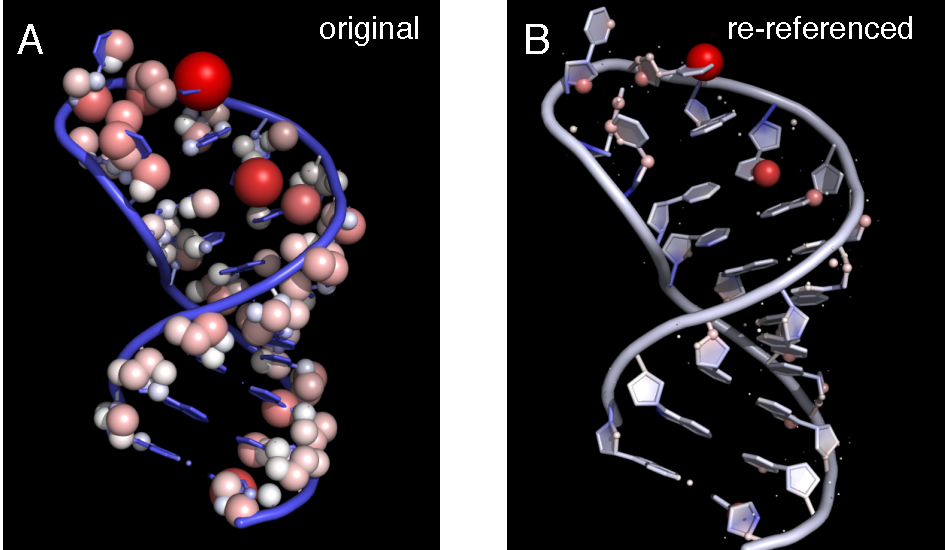
\includegraphics[width=0.5\textwidth]{figure_supplement_referencing}
\end{center}
\caption{ Visualizing referencing errors using PyShifts. Figure illustrating how referencing errors in chemical shift data can be visualized by computing chemical shift errors and then projecting them onto structural models. Cartoon representation of a test RNA with known $^{13}$C referencing errors (A) before and (B) after re-referencing the chemical shift data. Figures were generated using our Pymol plugin, PyShifts.}
\label{fig:ref_errors}
\end{figure}

\renewcommand\thetable{S\arabic{table}}    
\setcounter{table}{0}    
\begin{table}[h]
\centering
\begin{threeparttable}
\begin{tabular}{c c c c c c}
\hline
\\
nucleus  & LARMOR$^{\rm D}$ & RAMSEY  & LARMOR$^{\rm D}$-RAMSEY\\
\\
\hline
\\
1    & 0.459 & 0.549 & 0.463  \\
2    & 0.188 & 0.243 & 0.175  \\
3    & 0.081 & 0.109 & 0.082  \\
4    & 0.037 & 0.050 & 0.036  \\
5    & 0.019 & 0.019 & 0.018  \\
6    & 0.010 & 0.009 & 0.008  \\
7    & 0.008 & 0.004 & 0.004  \\
8    & 0.008 & 0.003 & 0.003  \\
9    & 0.004 & 0.002 & 0.002  \\
10   & 0.002 & 0.001 & 0.002  \\
11   & 0.002 & 0.001 & 0.002  \\
12   & 0.002 & 0.001 & 0.001  \\
none & 0.000 & 0.000 & 0.000  \\
 \\
\hline
\end{tabular}
\end{threeparttable}
\caption{\label{tab:fraction_removed}  Quanitying the fraction of datapoints identified as outleirs at each error threshold. Listed are average fraction of outliers identify at each error threshold. This average was calculated over the five RNAs in our testing set.}
\end{table}

\end{document}

